\documentclass[11pt,a4paper,notitlepage,onecolumn]{article}
\usepackage[german]{babel}
\usepackage[utf8]{inputenc}
\usepackage{graphicx}
\title{Aufgabe2\_3}
\author{Robin Nehls, Yves Müller\\
  Freie Universit\"at Berlin\\
  nehls@spline.de uves@spline.de }
\date{}
\begin{document}

\maketitle

\paragraph{} The first chart shows the values of the two summations, by 
using {\em double} and {\em long long integer} variables. As we can see
there is no noticable difference between the values of 
$S_{(up)}$, $S_{(down)}$ and the approximated value 
of the harmonic series.

\begin{figure}[!h]
\centering
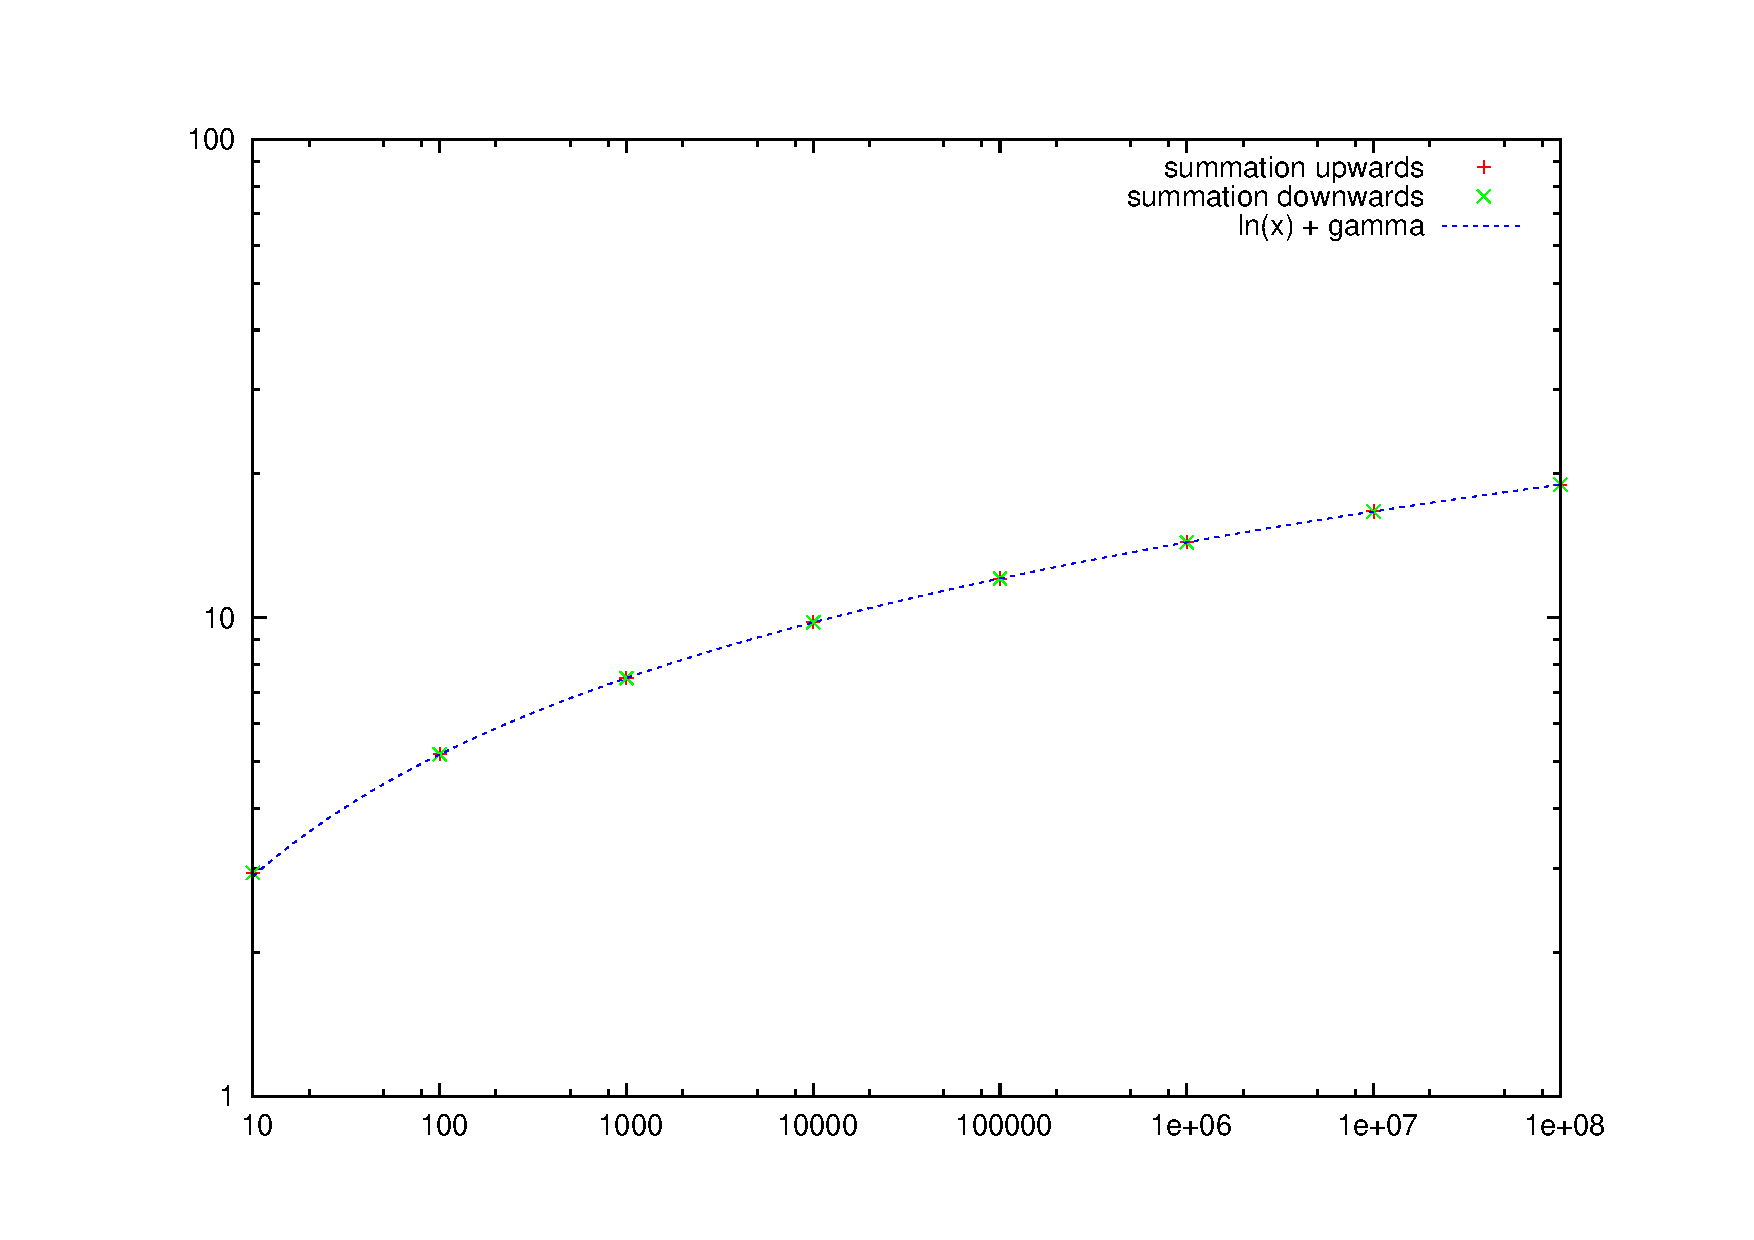
\includegraphics[width=0.8\textwidth]{aufgabe2-3-double.pdf}
\caption{\em \small Values using double precision}
\end{figure}

\paragraph{} Since it seems to be the taks to find differences between the 
two summation methods, we modified our programm to use {\em float} (but 
keept {\em long long integer} so we cloud use Ns higher then $10^{8}$

\begin{figure}
\centering
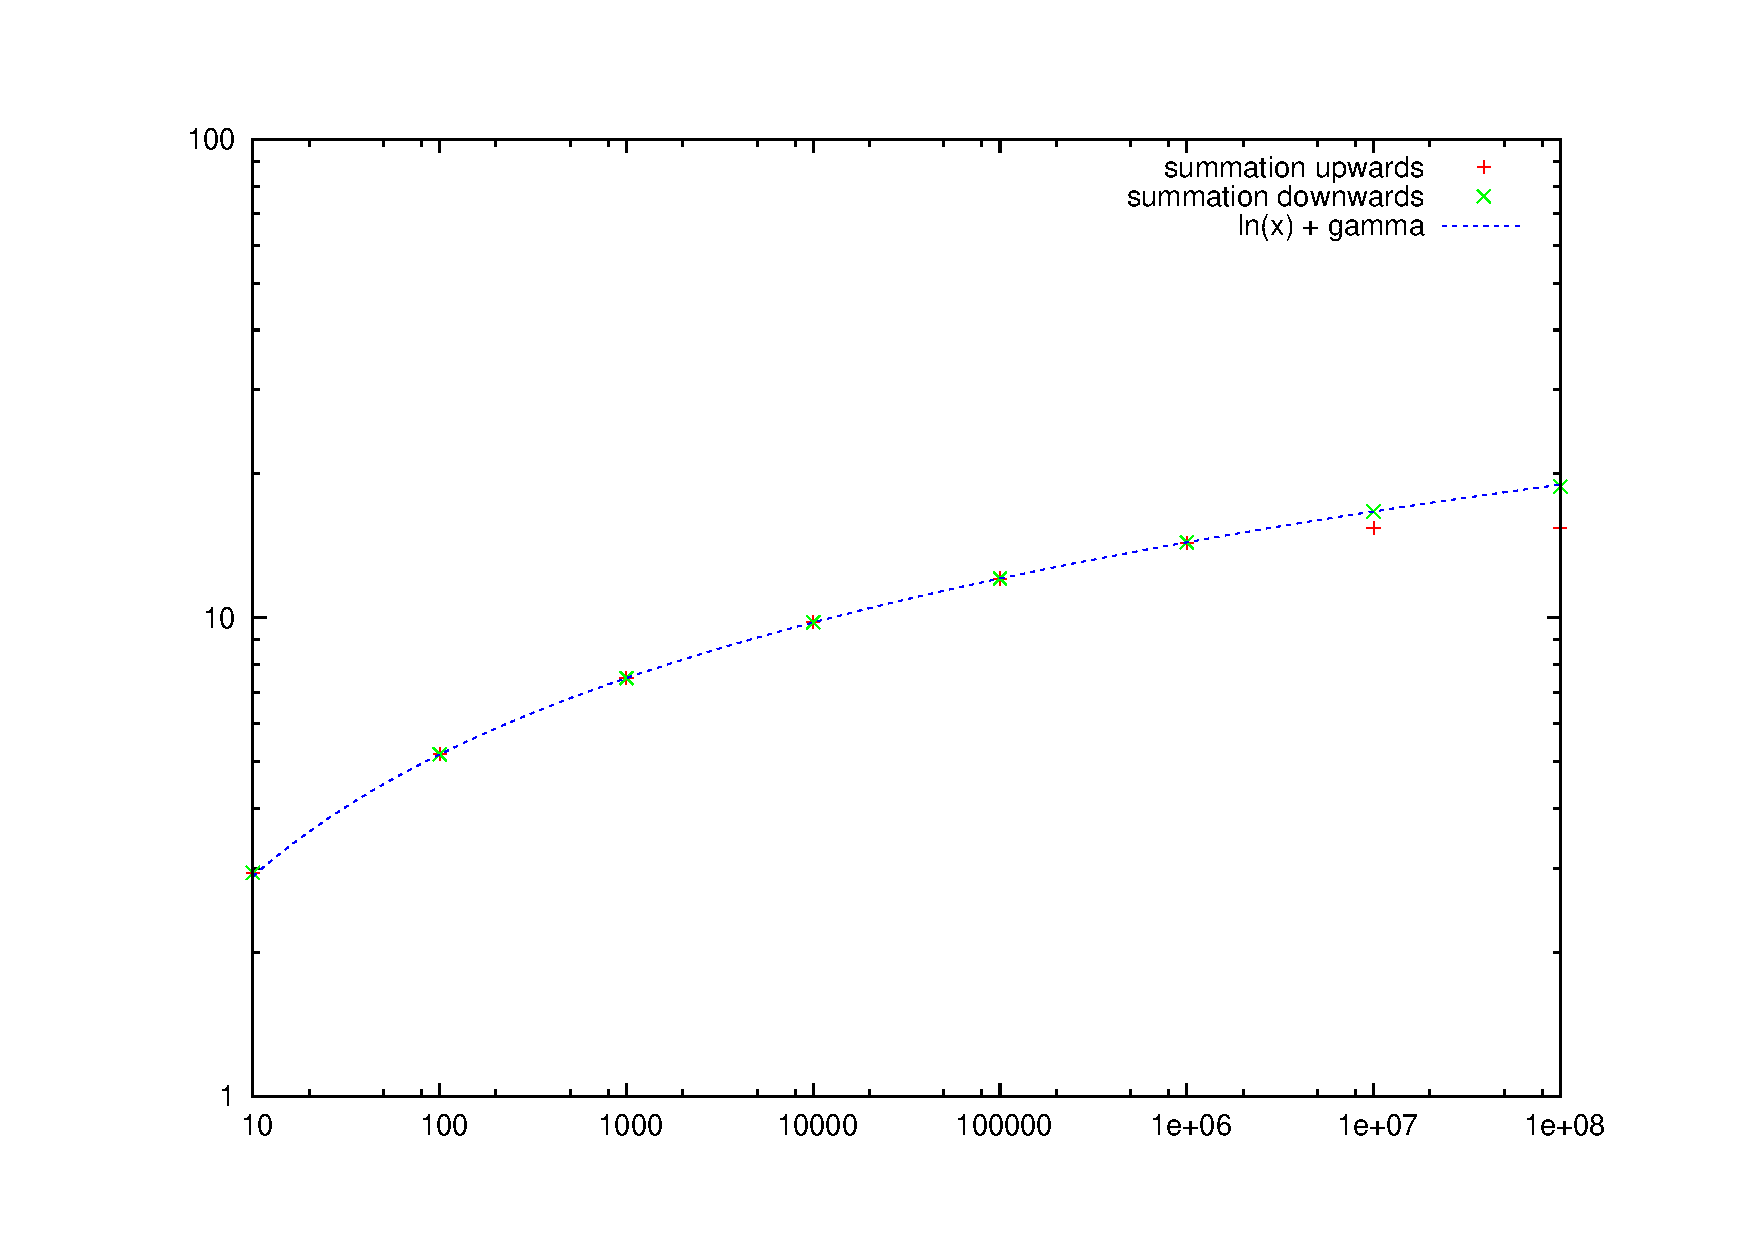
\includegraphics[width=0.8\textwidth]{aufgabe2-3-float.pdf}
\caption{\em \small Values using singel precision}
\end{figure}

\paragraph{} It seems that the summation from N to 1 is more precise than
the other method. As we saw in the previous assignment, the floating point
operations have more precise results when done with smaller numbers. By 
summing up from N to 1 the numbers added become bigger, so the operations
are always as much precise as both operands, while the other way round 
small values can easiely be lost by adding them to a much bigger number.

\begin{figure}
\centering
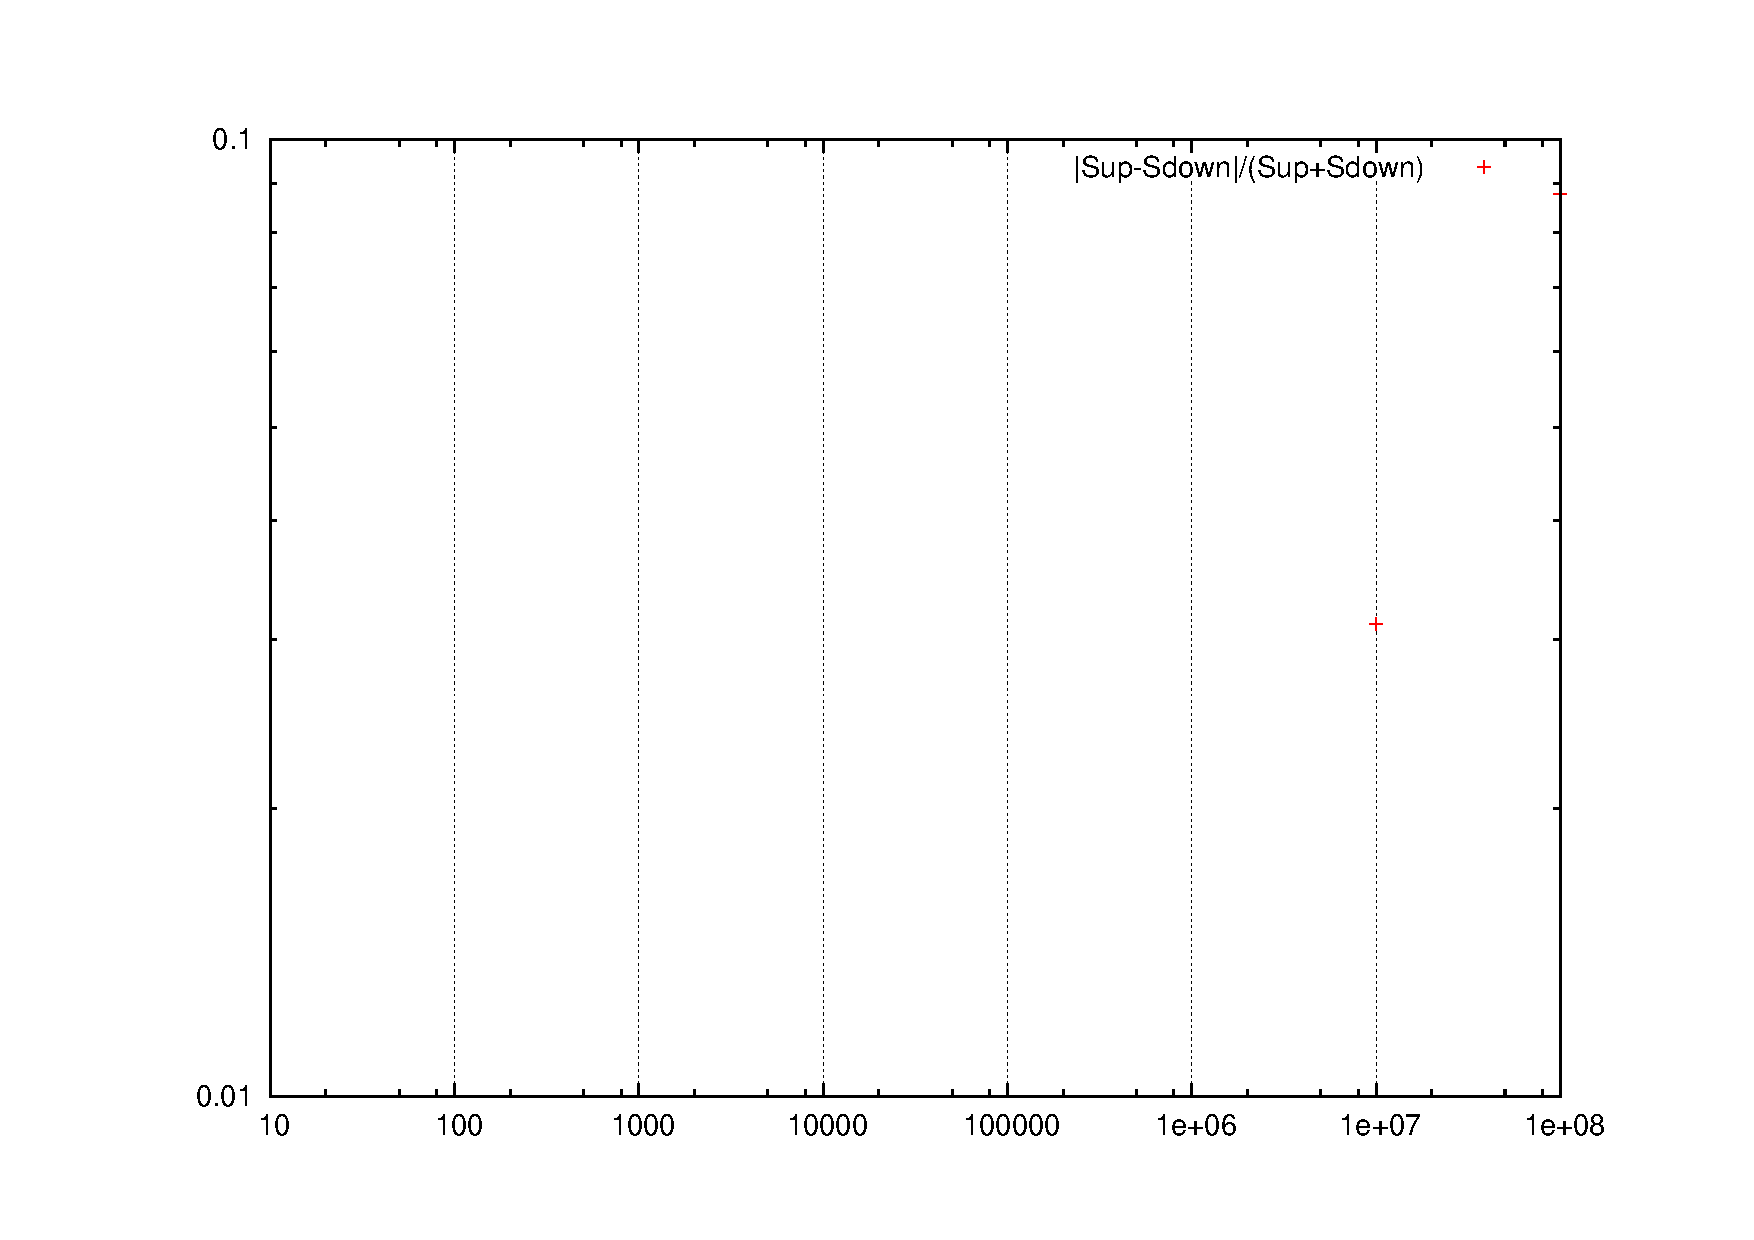
\includegraphics[width=0.8\textwidth]{aufgabe2-3-div.pdf}
\caption{\em \small desired plot}
\end{figure}

\paragraph{} On the last plot not much can be seen, since the values of
$S_{(up)}$ and $S_{(down)}$ only differ when N is greater then $10^7$.

\end{document}
